\documentclass[11pt]{article}
\usepackage[a4paper,margin=2.0cm]{geometry}
\usepackage[T1]{fontenc}
\usepackage{lmodern}
\usepackage{booktabs}
\usepackage{tabularx}
\usepackage{array}
\usepackage{threeparttable}
\usepackage{graphicx}
\usepackage{rotating}
\usepackage[table]{xcolor}
\usepackage[font=small,labelfont=bf]{caption}
\usepackage{pgfplots}
\usepgfplotslibrary{statistics}
\pgfplotsset{compat=1.18}
\definecolor{cmpPB}{RGB}{235,104,52}
\definecolor{cmpOther}{RGB}{42,120,214}
\definecolor{ordA}{RGB}{134,182,239}
\definecolor{ordB}{RGB}{57,135,229}
\definecolor{ordC}{RGB}{37,106,191}
\definecolor{ordD}{RGB}{24,79,149}
\definecolor{ordE}{RGB}{13,54,107}
\definecolor{cmpGrey}{RGB}{160,159,150}
\definecolor{cmpLight}{RGB}{225,224,217}
\definecolor{cmpMid}{RGB}{195,194,183}
% Generated by: node qedrank/cli.js compare (2026-10-14T13:36:18.667Z). Do not edit by hand; rebuild instead.
% Citation keys follow qedrank/data/benchmark-literature.json (cite_key). In this standalone file
% \cite shows the key; delete the next line when the tables and figures go into the paper.
\renewcommand{\cite}[1]{[\texttt{#1}]}
\begin{document}

\section*{ProofBench compared with Lean benchmarks}
Statement statistics use one rule for every benchmark: Lean tokens of the theorem signature, and of the signature with every non-Mathlib definition it uses (same file or the benchmark's own library, followed transitively). Measured on source text, without elaboration.

\begin{sidewaystable}
\centering
\caption{Lean benchmarks for formal mathematics, as described by their authors. ProofBench as of commit \texttt{466b32a}.}
\label{tab:bench-characteristics}
\scriptsize
\begin{tabularx}{\linewidth}{@{}>{\raggedright\arraybackslash}p{2.3cm}r>{\raggedright\arraybackslash}p{2.2cm}>{\raggedright\arraybackslash}X>{\raggedright\arraybackslash}X>{\raggedright\arraybackslash}X>{\raggedright\arraybackslash}X>{\raggedright\arraybackslash}p{1.6cm}@{}}
\toprule
Benchmark & Problems & Proof assistant & Level & Problems from & Task & Judged by & Statements \\
\midrule
\textbf{ProofBench} & 111 & Lean 4 & Research level, including open problems & Recent research papers (mostly graph theory) & Prove the given statement (one sorry); disproof variants & Kernel replay; statement and challenge definitions unchanged; axioms propext, Classical.choice, Quot.sound only & private \\\addlinespace[2pt]
miniF2F \cite{zheng2022} & 488 & Lean (3, Lean 4 ports), Isabelle, HOL Light, Metamath & High-school competition and coursework & AMC, AIME, IMO, the MATH dataset, custom high-school and undergraduate problems & Prove the given statement (answers written into the statement) & No official protocol; each paper checks compilation itself & public \\\addlinespace[2pt]
PutnamBench \cite{tsoukalas2024} & 672 & Lean 4, Isabelle, Coq/Rocq & Undergraduate competition & Putnam competition, 1962--2025 & Prove the given statement; about 60\% need an exhibited answer (with or without the answer supplied) & Compiles against the repository statements; results need a preprint & public \\\addlinespace[2pt]
FormalMATH \cite{yu2025} & 5{,}560 & Lean 4 & High-school olympiad to undergraduate & Omni-MATH, Numina-Olympiad, AIME, BlueMO, U-Math, HARDMath, DEMIMATH; autoformalized, filtered and expert-reviewed & Prove the given statement (answers embedded) & Lean 4 compiler (leanprover-community/repl) & public \\\addlinespace[2pt]
MSC-180 \cite{li2025} & 180 & Lean 4 & Undergraduate to graduate (graduate-dominant) & Undergraduate and graduate textbooks; autoformalized, then rewritten by hand & Prove the given statement & Compilation (kimina-lean-server) & public \\\addlinespace[2pt]
ProofNet \cite{azerbayev2023} & 371 & Lean 3 (Lean 4 ports) & Undergraduate & Textbook exercises (Rudin, Pugh, Stein--Shakarchi, Axler, Dummit--Foote, Herstein, Artin, Munkres, Ireland--Rosen) and Putnam & Theorem proving and (auto)formalization & No proving protocol defined in the paper & public \\\addlinespace[2pt]
CombiBench \cite{liu2025} & 100 & Lean 4 & Middle school to IMO and university & Hackmath, Brualdi's textbook, IMO and other olympiads & Prove; construct the answer first for 45 problems (Fine-Eval) & Fine-Eval: compiles, no sorry, no new axioms, statement unchanged, answer matches & public \\\addlinespace[2pt]
AMBER \cite{yang2026} & 200 & Lean 4 & Course exercises (easy) to PhD qualifying exams (hard) & Textbooks (Boyd--Vandenberghe, Golub--Van Loan, Vershynin) & Construct-then-prove (82 tasks) and prove (118) & Definition and proof compile within k samples & no public release found \\\addlinespace[2pt]
FormalProofBench \cite{ravi2026} & 200 & Lean 4 & Advanced undergraduate and graduate & Qualifying exams and textbooks, formalized by Lean experts & Prove the given statement (agentic, up to 40 turns) & Kernel accepts; \#print axioms, no sorryAx; native\_decide accepted & private (samples public) \\\addlinespace[2pt]
LeanEval & 128 & Lean 4 & Hard, research-level formalization (mostly not open problems) & Community-submitted, reviewed statements; Imperial College Annals Challenge corpus & Prove trusted statements; some problems also ask for definitions or instances & comparator: same statement, permitted axioms only, kernel check & public \\\addlinespace[2pt]
\bottomrule
\end{tabularx}
\end{sidewaystable}

\begin{table}[!htbp]
\centering
\begin{threeparttable}
\caption{Best reported results and statement complexity. Statement measures are computed here with one rule for every benchmark.}
\label{tab:bench-measured}
\scriptsize
\begin{tabular}{@{}l r >{\raggedright\arraybackslash}p{2.6cm} >{\raggedright\arraybackslash}p{1.7cm} r r r@{}}
\toprule
 & \multicolumn{3}{c}{Best reported\tnote{a}} & \multicolumn{3}{c}{Statement\tnote{b}} \\
\cmidrule(lr){2-4}\cmidrule(l){5-7}
Benchmark & Success & Model & Budget & Signature & With definitions [IQR] & Own definitions \\
\midrule
\textbf{ProofBench} & 0/80 (0.0\,\%) & Qwen3 30B-A3B Instruct & pass@1 & 43 & 293 {\footnotesize[118, 501]} & 95/111 (86\,\%) \\
miniF2F & 99.6\,\% & Seed-Prover & refinement, pass@8--16 & 41 & 41 {\footnotesize[27, 58]} & 0/488 (0\,\%) \\
PutnamBench & 100.0\,\% & Aleph Prover and 3 others & avg \$74 per problem & 87 & 92 {\footnotesize[69, 130]} & 9/672 (1\,\%) \\
FormalMATH & 28.3\,\% & DeepSeek-Prover-V2-671B & pass@32 & 62 & 65 {\footnotesize[46, 89]} & 626/5558 (11\,\%) \\
MSC-180 & 18.9\,\% & DeepSeek-Prover-V2-7B & pass@32 & 63 & 83 {\footnotesize[54, 116]} & 41/180 (23\,\%) \\
ProofNet & 37.1\,\% & DeepSeek-Prover-V2-671B & pass@1024 & 48 & 49 {\footnotesize[32, 65]} & 12/371 (3\,\%) \\
CombiBench & 30.0\,\% & Seed-Prover & refinement & 41 & 105 {\footnotesize[58, 191]} & 57/100 (57\,\%) \\
AMBER & 6.0\,\% & DeepSeek-V3.2 / Gemini-3.0 Pro & pass@16 & \multicolumn{3}{c}{\footnotesize not measured} \\
FormalProofBench & 100.0\,\% & 4 systems (tie) & one agentic run & \multicolumn{3}{c}{\footnotesize not measured} \\
LeanEval & 69.5\,\% & Axiom Prover & open submissions & 49 & 132 {\footnotesize[74, 297]} & 88/128 (69\,\%) \\
\bottomrule
\end{tabular}
\begin{tablenotes}\footnotesize
\item[a] As reported by the benchmark's paper or leaderboard; rates are comparable only at equal sampling budget. ProofBench: QEDRank runs, verified answers over established main theorems with a determinate outcome.
\item[b] Median Lean tokens of the theorem signature, and of the signature together with every non-Mathlib definition it uses (same file or the benchmark's own library, transitively); share of problems whose statement uses at least one such definition.
\end{tablenotes}
\end{threeparttable}
\end{table}

\begin{figure}[!htbp]
\centering
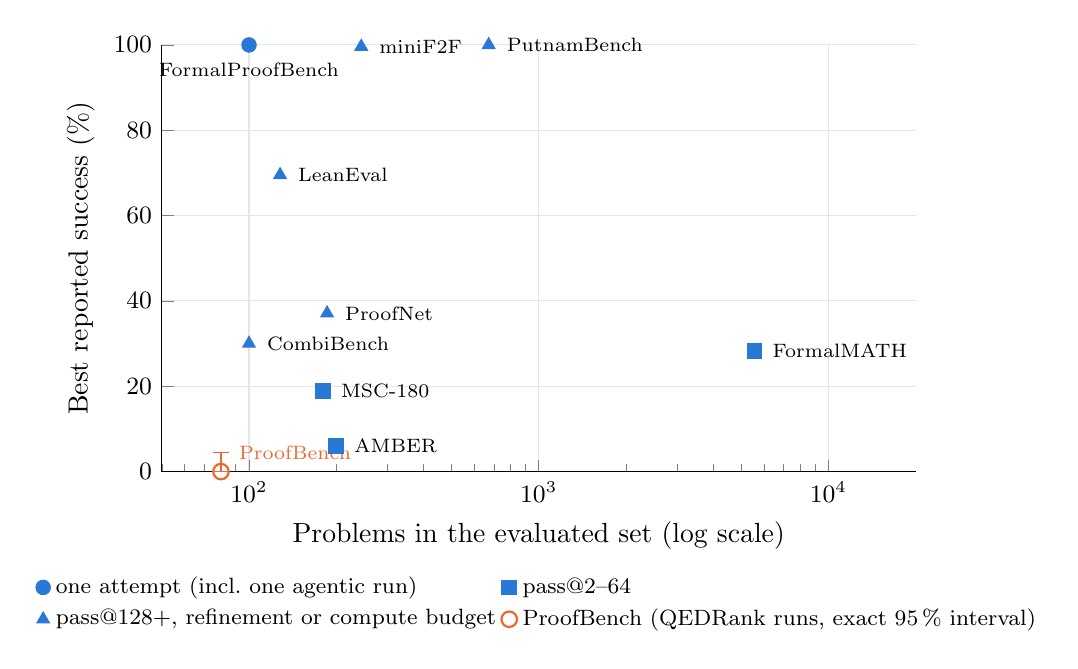
\begin{tikzpicture}
\begin{semilogxaxis}[
  width=0.92\linewidth, height=7cm, xmin=50, xmax=20000, ymin=0, ymax=100,
  xlabel={Problems in the evaluated set (log scale)}, ylabel={Best reported success (\%)},
  grid=major, grid style={draw=black!10}, axis lines*=left, tick label style={font=\small},
  legend style={at={(0.5,-0.22)}, anchor=north, legend columns=2, draw=none, font=\footnotesize},
  legend cell align=left, clip=false,
]
\addplot[only marks, mark=*, mark size=2.6pt, color=cmpOther] coordinates {(100,100.00)};
\addplot[only marks, mark=square*, mark size=2.6pt, color=cmpOther] coordinates {(5560,28.31) (180,18.89) (200,6.00)};
\addplot[only marks, mark=triangle*, mark size=2.6pt, color=cmpOther] coordinates {(244,99.60) (672,100.00) (186,37.10) (100,30.00) (128,69.53)};
\addplot[only marks, mark=o, mark size=2.8pt, color=cmpPB, thick, error bars/.cd, y dir=both, y explicit, error bar style={color=cmpPB, thick}] coordinates {(80,0.00) += (0,4.51) -= (0,0.00)};
\node[font=\scriptsize, anchor=north, yshift=-3pt, text=black] at (axis cs:100,100.00) {FormalProofBench};
\node[font=\scriptsize, anchor=west, xshift=3pt, text=black] at (axis cs:5560,28.31) {FormalMATH};
\node[font=\scriptsize, anchor=west, xshift=3pt, text=black] at (axis cs:180,18.89) {MSC-180};
\node[font=\scriptsize, anchor=west, xshift=3pt, text=black] at (axis cs:200,6.00) {AMBER};
\node[font=\scriptsize, anchor=west, xshift=3pt, text=black] at (axis cs:244,99.60) {miniF2F};
\node[font=\scriptsize, anchor=west, xshift=3pt, text=black] at (axis cs:672,100.00) {PutnamBench};
\node[font=\scriptsize, anchor=west, xshift=3pt, text=black] at (axis cs:186,37.10) {ProofNet};
\node[font=\scriptsize, anchor=west, xshift=3pt, text=black] at (axis cs:100,30.00) {CombiBench};
\node[font=\scriptsize, anchor=west, xshift=3pt, text=black] at (axis cs:128,69.53) {LeanEval};
\node[font=\scriptsize, anchor=west, xshift=3pt, text=cmpPB] at (axis cs:80,4.51) {ProofBench};
\legend{{one attempt (incl.\ one agentic run)},{pass@2--64},{pass@128+, refinement or compute budget},{ProofBench (QEDRank runs, exact 95\,\% interval)}}
\end{semilogxaxis}
\end{tikzpicture}
\caption{Headroom against size. Each benchmark at its best verified result, placed at the size of the set that result was reported on; marker shape gives the budget behind the number. ProofBench is shown with its exact 95\,\% Clopper--Pearson interval from the QEDRank runs.}
\label{fig:bench-headroom}
\end{figure}

\begin{figure}[!htbp]
\centering
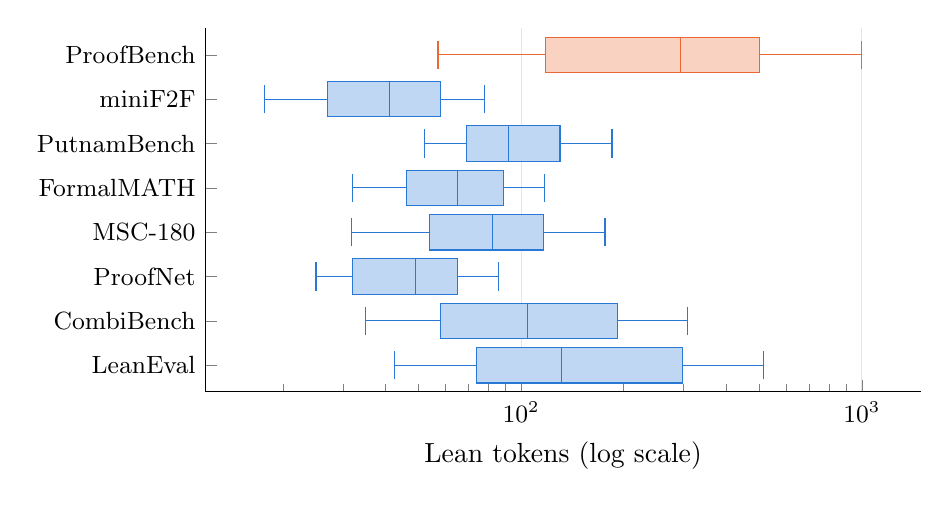
\begin{tikzpicture}
\begin{axis}[
  boxplot/draw direction=x, xmode=log, width=0.88\linewidth, height=6.2cm,
  ytick={8,7,6,5,4,3,2,1}, yticklabels={ProofBench,miniF2F,PutnamBench,FormalMATH,MSC-180,ProofNet,CombiBench,LeanEval},
  ymin=0.4, ymax=8.6, xlabel={Lean tokens (log scale)}, xmajorgrids, grid style={draw=black!10},
  tick label style={font=\small}, axis lines*=left,
]
\addplot[cmpPB, fill=cmpPB!30, boxplot prepared={lower whisker=57.0, lower quartile=118.0, median=293.0, upper quartile=501.0, upper whisker=996.0, draw position=8}] coordinates {};
\addplot[cmpOther, fill=cmpOther!30, boxplot prepared={lower whisker=17.7, lower quartile=27.0, median=41.0, upper quartile=58.0, upper whisker=78.3, draw position=7}] coordinates {};
\addplot[cmpOther, fill=cmpOther!30, boxplot prepared={lower whisker=52.0, lower quartile=69.0, median=92.0, upper quartile=130.0, upper whisker=184.8, draw position=6}] coordinates {};
\addplot[cmpOther, fill=cmpOther!30, boxplot prepared={lower whisker=32.0, lower quartile=46.0, median=65.0, upper quartile=89.0, upper whisker=117.0, draw position=5}] coordinates {};
\addplot[cmpOther, fill=cmpOther!30, boxplot prepared={lower whisker=31.8, lower quartile=53.8, median=82.5, upper quartile=116.3, upper whisker=176.3, draw position=4}] coordinates {};
\addplot[cmpOther, fill=cmpOther!30, boxplot prepared={lower whisker=25.0, lower quartile=32.0, median=49.0, upper quartile=65.0, upper whisker=86.0, draw position=3}] coordinates {};
\addplot[cmpOther, fill=cmpOther!30, boxplot prepared={lower whisker=35.0, lower quartile=58.0, median=104.5, upper quartile=191.3, upper whisker=308.3, draw position=2}] coordinates {};
\addplot[cmpOther, fill=cmpOther!30, boxplot prepared={lower whisker=42.5, lower quartile=73.8, median=131.5, upper quartile=297.0, upper whisker=514.9, draw position=1}] coordinates {};
\end{axis}
\end{tikzpicture}
\caption{Statement length including the definitions the theorem uses. Box: middle half of the problems; bar: median; whiskers: 10th to 90th percentile.}
\label{fig:bench-closure}
\end{figure}

\begin{figure}[!htbp]
\centering
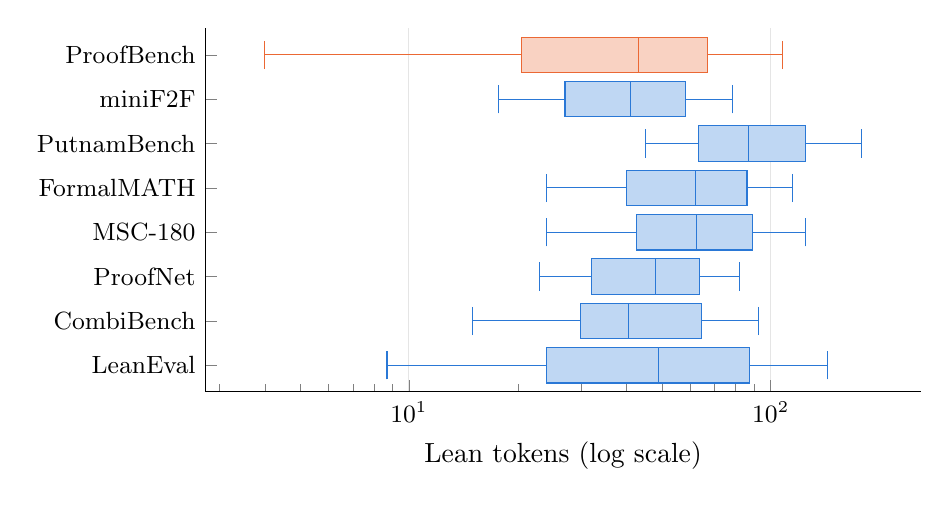
\begin{tikzpicture}
\begin{axis}[
  boxplot/draw direction=x, xmode=log, width=0.88\linewidth, height=6.2cm,
  ytick={8,7,6,5,4,3,2,1}, yticklabels={ProofBench,miniF2F,PutnamBench,FormalMATH,MSC-180,ProofNet,CombiBench,LeanEval},
  ymin=0.4, ymax=8.6, xlabel={Lean tokens (log scale)}, xmajorgrids, grid style={draw=black!10},
  tick label style={font=\small}, axis lines*=left,
]
\addplot[cmpPB, fill=cmpPB!30, boxplot prepared={lower whisker=4.0, lower quartile=20.5, median=43.0, upper quartile=67.0, upper whisker=108.0, draw position=8}] coordinates {};
\addplot[cmpOther, fill=cmpOther!30, boxplot prepared={lower whisker=17.7, lower quartile=27.0, median=41.0, upper quartile=58.0, upper whisker=78.3, draw position=7}] coordinates {};
\addplot[cmpOther, fill=cmpOther!30, boxplot prepared={lower whisker=45.1, lower quartile=63.0, median=87.0, upper quartile=125.0, upper whisker=177.9, draw position=6}] coordinates {};
\addplot[cmpOther, fill=cmpOther!30, boxplot prepared={lower whisker=24.0, lower quartile=40.0, median=62.0, upper quartile=86.0, upper whisker=115.0, draw position=5}] coordinates {};
\addplot[cmpOther, fill=cmpOther!30, boxplot prepared={lower whisker=24.0, lower quartile=42.5, median=62.5, upper quartile=89.0, upper whisker=124.8, draw position=4}] coordinates {};
\addplot[cmpOther, fill=cmpOther!30, boxplot prepared={lower whisker=23.0, lower quartile=32.0, median=48.0, upper quartile=63.5, upper whisker=82.0, draw position=3}] coordinates {};
\addplot[cmpOther, fill=cmpOther!30, boxplot prepared={lower whisker=15.0, lower quartile=29.8, median=40.5, upper quartile=64.5, upper whisker=92.7, draw position=2}] coordinates {};
\addplot[cmpOther, fill=cmpOther!30, boxplot prepared={lower whisker=8.7, lower quartile=24.0, median=49.0, upper quartile=87.3, upper whisker=143.3, draw position=1}] coordinates {};
\end{axis}
\end{tikzpicture}
\caption{Length of the theorem signature alone. Box: middle half of the problems; bar: median; whiskers: 10th to 90th percentile.}
\label{fig:bench-signature}
\end{figure}

\begin{table}[!htbp]
\centering
\caption{Subject coverage: share of labelled problems (\%) by subject area; a problem with several labels counts in each. Logic: logic and foundations; Combinatorics: combinatorics and discrete mathematics; Analysis: analysis and calculus; Geometry/topology: geometry and topology; Probability: probability and statistics; Applied: applied mathematics, physics and optimization. $^{*}$: counts stated in the benchmark's paper.}
\label{tab:bench-subjects}
\scriptsize
\setlength{\tabcolsep}{3pt}
\begin{tabular}{@{}lcccccccccr@{}}
\toprule
Benchmark & \rotatebox{60}{Logic} & \rotatebox{60}{Combinatorics} & \rotatebox{60}{Number theory} & \rotatebox{60}{Algebra} & \rotatebox{60}{Analysis} & \rotatebox{60}{Geometry/topology} & \rotatebox{60}{Probability} & \rotatebox{60}{Applied} & \rotatebox{60}{Other} & $n$ \\
\midrule
\textbf{ProofBench} & \cellcolor{cmpOther!9}{1} & \cellcolor{cmpOther!71}\textcolor{white}{87} & \cellcolor{cmpOther!11}{5} & \cellcolor{cmpOther!10}{3} & \cellcolor{white}\textcolor{black!35}{0} & \cellcolor{cmpOther!11}{4} & \cellcolor{cmpOther!9}{1} & \cellcolor{white}\textcolor{black!35}{0} & \cellcolor{white}\textcolor{black!35}{0} & 110 \\
miniF2F & \cellcolor{white}\textcolor{black!35}{0} & \cellcolor{white}\textcolor{black!35}{0} & \cellcolor{cmpOther!39}{43} & \cellcolor{cmpOther!49}\textcolor{white}{57} & \cellcolor{white}\textcolor{black!35}{0} & \cellcolor{white}\textcolor{black!35}{0} & \cellcolor{white}\textcolor{black!35}{0} & \cellcolor{white}\textcolor{black!35}{0} & \cellcolor{white}\textcolor{black!35}{0} & 313 \\
PutnamBench & \cellcolor{cmpOther!9}{1} & \cellcolor{cmpOther!11}{4} & \cellcolor{cmpOther!18}{13} & \cellcolor{cmpOther!38}{42} & \cellcolor{cmpOther!30}{30} & \cellcolor{cmpOther!14}{8} & \cellcolor{cmpOther!9}{1} & \cellcolor{white}\textcolor{black!35}{0} & \cellcolor{white}\textcolor{black!35}{0} & 672 \\
FormalMATH & \cellcolor{white}\textcolor{black!35}{0} & \cellcolor{cmpOther!14}{8} & \cellcolor{cmpOther!23}{20} & \cellcolor{cmpOther!42}{47} & \cellcolor{cmpOther!16}{11} & \cellcolor{cmpOther!12}{5} & \cellcolor{white}\textcolor{black!35}{0} & \cellcolor{cmpOther!14}{8} & \cellcolor{cmpOther!8}{$<$1} & 5560 \\
MSC-180 & \cellcolor{cmpOther!9}{2} & \cellcolor{cmpOther!10}{3} & \cellcolor{cmpOther!9}{2} & \cellcolor{cmpOther!22}{20} & \cellcolor{cmpOther!31}{32} & \cellcolor{cmpOther!16}{12} & \cellcolor{cmpOther!10}{3} & \cellcolor{cmpOther!27}{27} & \cellcolor{white}\textcolor{black!35}{0} & 180 \\
ProofNet & \cellcolor{white}\textcolor{black!35}{0} & \cellcolor{white}\textcolor{black!35}{0} & \cellcolor{cmpOther!12}{6} & \cellcolor{cmpOther!46}{53} & \cellcolor{cmpOther!26}{25} & \cellcolor{cmpOther!20}{17} & \cellcolor{white}\textcolor{black!35}{0} & \cellcolor{white}\textcolor{black!35}{0} & \cellcolor{white}\textcolor{black!35}{0} & 359 \\
CombiBench & \cellcolor{white}\textcolor{black!35}{0} & \cellcolor{cmpOther!80}\textcolor{white}{100} & \cellcolor{white}\textcolor{black!35}{0} & \cellcolor{white}\textcolor{black!35}{0} & \cellcolor{white}\textcolor{black!35}{0} & \cellcolor{white}\textcolor{black!35}{0} & \cellcolor{white}\textcolor{black!35}{0} & \cellcolor{white}\textcolor{black!35}{0} & \cellcolor{white}\textcolor{black!35}{0} & 100 \\
AMBER$^{*}$ & \cellcolor{white}\textcolor{black!35}{0} & \cellcolor{white}\textcolor{black!35}{0} & \cellcolor{white}\textcolor{black!35}{0} & \cellcolor{white}\textcolor{black!35}{0} & \cellcolor{cmpOther!26}{25} & \cellcolor{white}\textcolor{black!35}{0} & \cellcolor{cmpOther!26}{25} & \cellcolor{cmpOther!44}{50} & \cellcolor{white}\textcolor{black!35}{0} & 200 \\
FormalProofBench$^{*}$ & \cellcolor{cmpOther!16}{11} & \cellcolor{white}\textcolor{black!35}{0} & \cellcolor{cmpOther!16}{12} & \cellcolor{cmpOther!22}{20} & \cellcolor{cmpOther!38}{41} & \cellcolor{white}\textcolor{black!35}{0} & \cellcolor{cmpOther!20}{17} & \cellcolor{white}\textcolor{black!35}{0} & \cellcolor{white}\textcolor{black!35}{0} & 200 \\
LeanEval & \cellcolor{cmpOther!9}{2} & \cellcolor{cmpOther!14}{8} & \cellcolor{cmpOther!28}{28} & \cellcolor{cmpOther!20}{16} & \cellcolor{cmpOther!17}{13} & \cellcolor{cmpOther!31}{32} & \cellcolor{white}\textcolor{black!35}{0} & \cellcolor{cmpOther!9}{1} & \cellcolor{cmpOther!9}{1} & 128 \\
\bottomrule
\end{tabular}
\end{table}

\begin{figure}[!htbp]
\centering
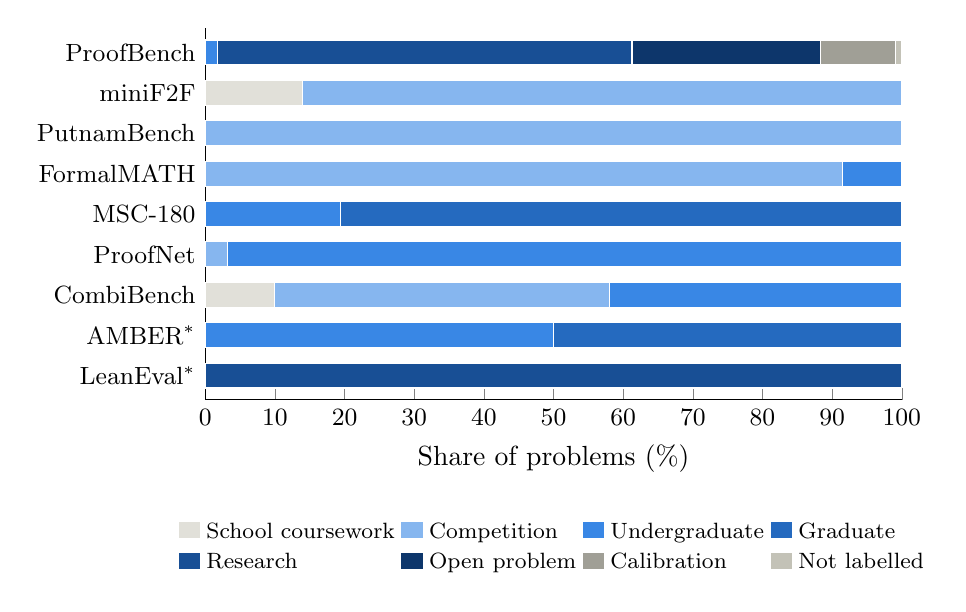
\begin{tikzpicture}
\begin{axis}[
  xbar stacked, bar width=9pt, width=0.86\linewidth, height=6.3cm, xmin=0, xmax=100,
  xlabel={Share of problems (\%)}, ytick={0,1,2,3,4,5,6,7,8},
  yticklabels={LeanEval$^{*}$,AMBER$^{*}$,CombiBench,ProofNet,MSC-180,FormalMATH,PutnamBench,miniF2F,ProofBench},
  ymin=-0.6, ymax=8.6, tick label style={font=\small}, axis lines*=left,
  legend style={at={(0.5,-0.3)}, anchor=north, legend columns=4, draw=none, font=\footnotesize}, legend cell align=left,
]
\addplot[fill=cmpLight, draw=white] coordinates {(0.00,8) (13.93,7) (0.00,6) (0.00,5) (0.00,4) (0.00,3) (10.00,2) (0.00,1) (0.00,0)};
\addplot[fill=ordA, draw=white] coordinates {(0.00,8) (86.07,7) (100.00,6) (91.53,5) (0.00,4) (3.23,3) (48.00,2) (0.00,1) (0.00,0)};
\addplot[fill=ordB, draw=white] coordinates {(1.80,8) (0.00,7) (0.00,6) (8.47,5) (19.44,4) (96.77,3) (42.00,2) (50.00,1) (0.00,0)};
\addplot[fill=ordC, draw=white] coordinates {(0.00,8) (0.00,7) (0.00,6) (0.00,5) (80.56,4) (0.00,3) (0.00,2) (50.00,1) (0.00,0)};
\addplot[fill=ordD, draw=white] coordinates {(59.46,8) (0.00,7) (0.00,6) (0.00,5) (0.00,4) (0.00,3) (0.00,2) (0.00,1) (100.00,0)};
\addplot[fill=ordE, draw=white] coordinates {(27.03,8) (0.00,7) (0.00,6) (0.00,5) (0.00,4) (0.00,3) (0.00,2) (0.00,1) (0.00,0)};
\addplot[fill=cmpGrey, draw=white] coordinates {(10.81,8) (0.00,7) (0.00,6) (0.00,5) (0.00,4) (0.00,3) (0.00,2) (0.00,1) (0.00,0)};
\addplot[fill=cmpMid, draw=white] coordinates {(0.90,8) (0.00,7) (0.00,6) (0.00,5) (0.00,4) (0.00,3) (0.00,2) (0.00,1) (0.00,0)};
\legend{{School coursework},{Competition},{Undergraduate},{Graduate},{Research},{Open problem},{Calibration},{Not labelled}}
\end{axis}
\end{tikzpicture}
\caption{Problems by level. Per-problem labels where the benchmark has them; $^{*}$: level or counts stated by the benchmark's authors. No level breakdown published: FormalProofBench.}
\label{fig:bench-levels}
\end{figure}

\begin{figure}[!htbp]
\centering
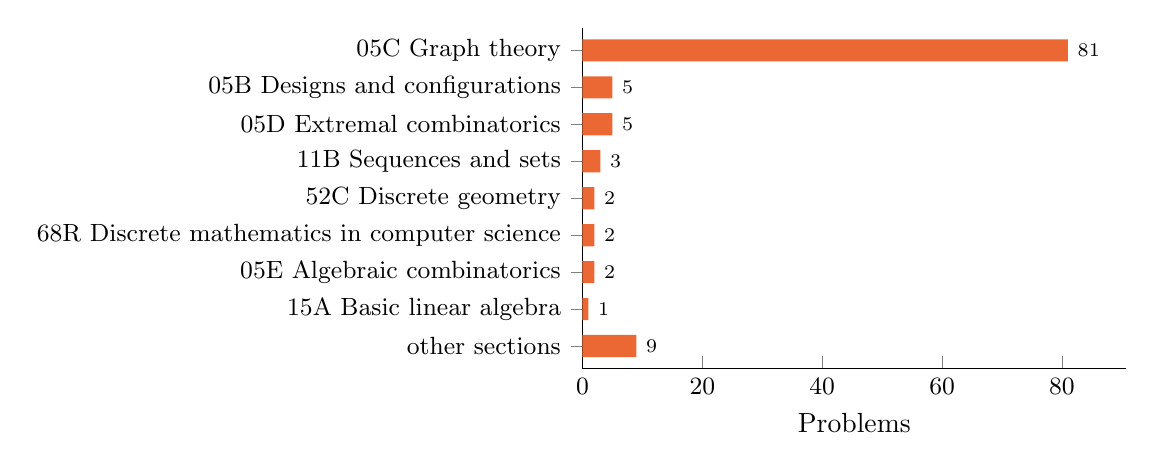
\begin{tikzpicture}
\begin{axis}[
  xbar, bar width=8pt, width=0.7\linewidth, height=5.9cm, xmin=0,
  xlabel={Problems}, ytick={0,1,2,3,4,5,6,7,8}, yticklabels={other sections,15A Basic linear algebra,05E Algebraic combinatorics,68R Discrete mathematics in computer science,52C Discrete geometry,11B Sequences and sets,05D Extremal combinatorics,05B Designs and configurations,05C Graph theory},
  ymin=-0.6, ymax=8.6, nodes near coords, nodes near coords style={font=\scriptsize},
  tick label style={font=\small}, axis lines*=left, enlarge x limits={upper, value=0.12},
]
\addplot[fill=cmpPB, draw=none] coordinates {(9,0) (1,1) (2,2) (2,3) (2,4) (3,5) (5,6) (5,7) (81,8)};
\end{axis}
\end{tikzpicture}
\caption{ProofBench problems by MSC~2020 section of their primary subject code (111 problems, 1 without a code).}
\label{fig:proofbench-msc}
\end{figure}

\end{document}
